%!TEX root = /Users/louis/Documents/PhD/Deliverables/Thesis/thesis.tex

\chapter{Review of Software Evolution}
\label{LiteratureReview}
This chapter reviews existing work on software evolution. In particular, this chapter explores the ways in which software evolution is identified and managed in the context of MDE, which was discussed in Chapter~\ref{Background}. Potential directions for future research are identified from the literature review, and Chapter~\ref{Analysis} performs a critical analysis of some of the tools and techniques reviewed in this chapter. The principles of software evolution are discussed in Section~\ref{sec:software_evolution_theory}, while Section~\ref{sec:software_evolution_practice} reviews the ways in which evolution is identified, analysed and managed in a range of fields, including relational databases, programming languages, and MDE development environments. From the review, Section~\ref{sec:literature_review_summary} synthesises research challenges for software evolution in the context of MDE, highlighting those to which this thesis contributes, and elaborates on the research method used in this thesis.

\section{Software Evolution Theory}
\label{sec:software_evolution_theory}
Software evolution is an important facet of software engineering. As discussed in Section~\ref{sec:intro_to_software_evo}, studies \cite{erlikh00leveraging,moad90maintaining} have shown that the evolution of software can account for as much as 90\% of a development budget, and there is no reason to believe the situation is different today. Such figures are sometimes described as uncertain \cite[ch. 21]{sommerville06software}, primarily because the term evolution is not used consistently. For example, some authors prefer the term \emph{maintenance} to \emph{evolution}. Here, the latter is preferred as the former can imply deterioration caused by repeated use, and most software systems do not deteriorate in this manner \cite{ramil00cost}. There is a corpus of software evolution research. Publications in this area have existed since the 1960s (e.g. \cite{lehman69programming}).

The remainder of this section introduces software evolution terminology and discusses three research areas that relate to software evolution: refactoring, design patterns and traceability. Refactoring concentrates on improving the structure of existing systems, design patterns on best practices for software design, and traceability for recording and analysing the lifecycle of software artefacts. Each area provides a vocabulary for discussing software design and evolution. There is an abundance of research in these areas, including seminal works on refactoring, such as \cite{opdyke92refactoring} and \cite{fowler99refactoring}; and on design patterns, such as \cite{gamma95patterns}.

\subsection{Categories of Software Evolution}
\label{subsec:categories_of_software_evolution}
Addressing \cc changing requirements, adapting to new technologies, and architectural restructuring have been identified as the primary reasons for software evolution \cite{sjoberg93quantifying}. These reasons are the motivations for three common types of software evolution \cite[ch. 21]{sommerville06software}:

\begin{itemize}
 \item \textbf{Corrective evolution} takes place when a system exhibiting unintended or faulty behaviour is corrected. Alternatively, corrective evolution may be used to adapt a system to new or changing requirements. 
 \item \textbf{Adaptive evolution} is employed to make a system compatible with a change to platforms or technologies that underpin its implementation.
 \item \textbf{Perfective evolution} refers to the process of improving the internal quality of a system, while preserving the behaviour of the system. 
\end{itemize}

The remainder of this section adopts this categorisation for discussing software evolution literature. Refactoring (discussed in Section~\ref{subsec:refactoring}), for instance, is one way in which perfective evolution can be realised.

\subsection{Evolutionary Development Activities}
Software evolution is identified and managed via many different development activities. Two \cc software evolution activities, \emph{impact analysis} (for reasoning about the effects of evolution) and \emph{change propagation} (for updating one artefact in response to a change made to another) are commonplace \cite{winkler09survey}. In \cc addition, \emph{reverse engineering} (analysing existing development artefacts to extract information) and \emph{source code translation} (rewriting code to use a more suitable technology, such as a different programming language) are also important software evolution activities \cite{sommerville06software}.

MDE introduces new software engineering principles, and  the concerns and requirements for software evolution differ between MDE processes and traditional software development processes. For example, MDE facilitates portable software by prescribing platform-independent and platform-specific models (as discussed in Section~\ref{sec:mde}), and as such source code translation is arguably less relevant to MDE than to traditional software engineering. Because MDE seeks to capture the essence of the software in models, reverse engineering information from, for example, code is also less likely to be relevant to MDE than to traditional software engineering. Consequently, this thesis focuses on impact analysis and change propagation, which are both relevant to MDE \cite{winkler09survey}, as discussed in Section~\ref{subsec:mde_evo}.

\subsection{Refactoring}
\label{subsec:refactoring}
There is ``an urgent need for techniques that reduce software complexity by incrementally improving the internal software quality'' \cite{mens04survey}. Refactoring is ``the process of changing a software system in such a way that it does not alter the external behaviour of the code yet improves its internal structure'' \cite[pg. xvi]{fowler99refactoring}. Refactoring plays a significant role in the evolution of software systems -- a recent study of five open-source projects showed that over 80\% of changes were refactorings \cite{dig06apis}.

Typically, refactoring literature concentrates on three primary activities in the refactoring process: \emph{identification} (where should refactoring be applied, and which refactorings should be used?), \emph{verification} (has refactoring preserved behaviour?) and \emph{assessment} (how has refactoring affected other qualities of the system, such as cohesion and efficiency?).

Beck describes an informal means for identifying the need for refactoring, termed \textit{bad smells}: ``structures in the code that suggest (sometimes scream for) the possibility of refactoring'' \cite[foreword]{fowler99refactoring}. Tools and semi-automated approaches have also been devised for refactoring identification, such as Daikon \cite{kataoka01automated}, which detects program invariants that may indicate the possibility for refactoring. Clone analysis tools have been employed for identifying refactorings that eliminate duplication \cite{balazinska00advanced,ducasse99language}. The types of refactoring being performed may vary over different domains. For example, Buck\footnote{In a keynote address to the First International Ruby on Rails Conference (RailsConf), May 2007, Portland, Oregon, United States of America.} describes refactorings, such as ``Skinny Controller, Fat Model'', particular to the Ruby on Rails web framework\footnote{\url{http://www.rubyonrails.org}}.

Since 2006, Dig has been studying the refactoring of systems that are developed by combining components, possibly developed by different organisations. The \cc changes made to five components that are known to have been re-used often were categorised, with the hypothesis that a significant number of the changes could be classified as behaviour-preserving (i.e. refactorings) \cite{dig06apis}. By using examples from the survey, an algorithm was devised for automatically detecting refactorings to a high degree of accuracy (over 85\%) \cite{dig06detection}. The algorithm was then utilised in tools for (1) replaying refactorings to perform migration of client code following breaking changes to a component \cite{dig06automatic}, and (2) versioning object-oriented programs using a refactoring-aware configuration management system \cite{dig07cms}. The latter facilitated better understanding of program evolution, and the refinement of the refactoring detection algorithm.


\subsection{Patterns and Anti-Patterns}
\label{sec:LitReviewPatterns}
A \textit{design pattern} identifies a commonly occurring design problem and describes a re-usable solution to that problem. Related design patterns are combined to form a \textit{pattern catalogue} -- such as for object-oriented programming \cite{gamma95patterns} or enterprise applications \cite{fowler02patterns}. A pattern description comprises at least a name, overview of the problem, and details of a common solution \cite{brown98antipatterns}. Depending on the domain, further information may be included in the pattern description (such as a classification, a description of the pattern's applicability and an example usage).

Design patterns can be thought of as describing objectives for improving the internal quality of a system (i.e. perfective software evolution). Often developers improve the quality of systems by restructing systems to exhibit design patterns \cite{kerievsky04refactoring}. Studying the way in which experts perform perfective software evolution can lead to devising best practices, sometimes in the form of a pattern catalogue, such as the object-oriented refactorings described in \cite{fowler99refactoring}.

Design \cc patterns were first used to devise a pattern catalogue for town planning \cite{alexander77pattern}. Refactorings \cc were later adapted to software architecture, by specifying a pattern catalogue for designing user-interfaces \cite{beck89constructing}. Utilising pattern catalogues allowed the software industry to ``reuse the expertise of experienced developers to repeatedly train the less experienced'' \cite[pg. 10]{brown98antipatterns}. Furthermore, \cc design patterns ``help to define a vocabulary for talking about software development and integration challenges; and provide a process for the orderly resolution of these challenges'' \cite[pg. xii]{rising01designpatterns}. 

Anti-patterns are an alternative literary form for describing patterns of a software architecture \cite{brown98antipatterns}. Rather than describe patterns that have often been observed in successful architectures, they describe those which are present in unsuccessful architectures. Essentially, an anti-pattern is a pattern in an inappropriate context, which describes a problematic solution to a frequently encountered problem. The (anti-)pattern catalogue may include alternative solutions that are known to yield better results (termed ``refactored solutions'' by Brown). Catalogues might also consider the reasons why (inexperienced) developers use an anti-pattern. Brown notes that ``patterns and anti-patterns are complementary'' \cite[pg. 13]{brown98antipatterns}; both are useful in providing a common vocabulary for discussion of system architectures and in educating less experienced developers.


\subsection{Traceability}
\label{subsec:traceability}
A software development artefact rarely evolves in isolation. Changes to one artefact cause and are caused by changes to other artefacts (e.g. object code is recompiled when source code changes, source code and documentation are updated when requirements change). Hence, traceability -- the ability to describe and follow the life of software artefacts \cite{winkler09survey,lago09scoped} -- is closely related to and facilitates software evolution.

Historically, traceability is a branch of requirements engineering, but is increasingly used for artefacts other than requirements \cite{winkler09survey}. Because MDE prescribes automated transformation between models, traceability is also researched in the context of MDE. The remainder of this section discusses traceability principles focussing on the relationship between traceability and software evolution. Section~\ref{subsec:mde_evo} reviews the traceability literature that relates to MDE.

The traceability literature uses inconsistent terminology. This thesis adopts the terminology described in a recent survey of traceability research \cite{winkler09survey}: \emph{traceability} is the ability to describe and follow the life of software artefacts; \emph{traceability links} are the relationships between software artefacts. Traceability is facilitated by traceability links, which document the dependencies, causalities and influences between artefacts. Traceability links are established by hand or by automated analysis of artefacts. In MDE environments, some traceability links can be automatically inferred because the relationships between some types of artefact are specified in a structured manner (for example, as a model-to-model transformation).

Traceability links are defined between artefacts at the same level of abstraction (horizontal links) and at different levels of abstraction (vertical links). Traceability links can be uni- or bi-directional. The former are navigated either \emph{forwards} (away from the dependent artefact) or \emph{backwards} (towards the dependent artefact). Figure~\ref{fig:traceability_links} summaries these categories of traceability link.

\begin{figure}[htbp]
  \begin{center}
    \leavevmode
    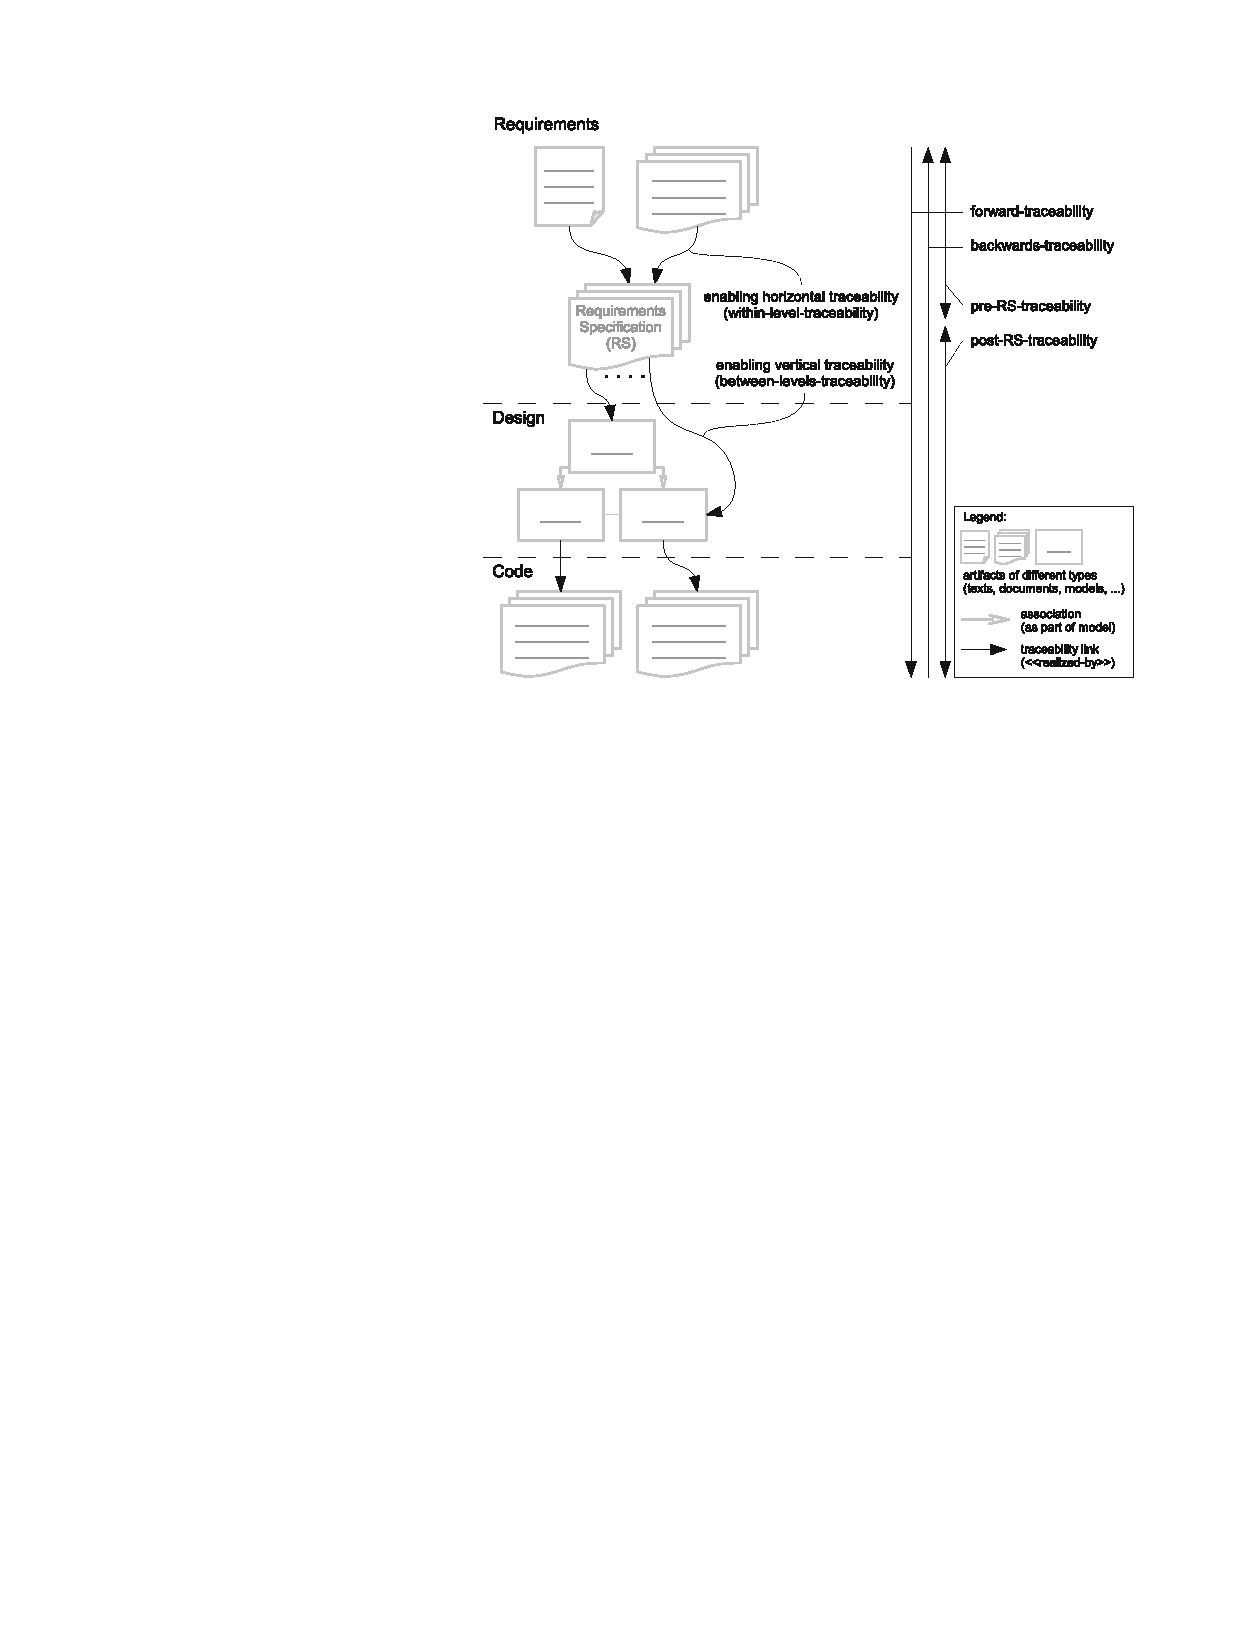
\includegraphics[width=11.5cm]{3.LiteratureReview/images/traceability_links.pdf}
  \end{center}
  \caption[Categories of traceability link]{Categories of traceability link \cite{winkler09survey}.}
  \label{fig:traceability_links}
\end{figure}

Traceability supports software evolution activities, such as impact analysis (discovering and reasoning about the effects of a change) and change propagation (updating impacted artefacts following a change to an artefact). Moreover, automated software evolution is facilitated by programmatic access to traceability links.

Current approaches for traceability-supported software evolution use \emph{triggers} and \emph{events}. Each approach proposes mechanisms for detecting triggers (changes to artefacts) and for notifying dependent artefacts of events (the details of a change). Existing approaches vary in the extent to which they can automatically update dependent artefacts. Some \cc approaches \cite{chen99consistency,cleland03eventbased} do not perform automatic updates, while others \cite{aizenbud05operational,costa2007rtmdd} provide guided or fully automatic updates. Section~\ref{subsubsec:model_synch} provides a more thorough discussion and critical analysis of event-based approaches for impact analysis and change propagation in the context of MDE.

To remain accurate and hence useful, traceability links must be updated as a system evolves. Although most existing approaches to traceability are ``not well suited to the evolution of [traceability] artefacts'' \cite[pg. 24]{winkler09survey}, there is some work in this area. For example, Mader et al. describe a development environment that records changes to artefacts, comparing the changes to a catalogue of built-in patterns \cite{mader08rule}. Each pattern provides an executable specification for updating traceability links.

Software evolution and traceability are entangled concerns. Traceability facilitates software evolution activities such as impact analysis and change propagation. Traceability is made possible with consistent and accurate traceability links. Software evolution can affect the relationships between artefacts (i.e. the traceability links) and hence software evolution techniques are applied to ensure that traceability links remain consistent and accurate.

\section{Software Evolution in Practice}
\label{sec:software_evolution_practice}
Using the principles of software evolution described above, this section examines the ways in which evolution is identified, managed and analysed in a variety of settings, including programming languages grammarware, relational database management system and MDE. 

\subsection{Programming Language Evolution}
Programming language designers often attempt to ensure that legacy programs continue to conform to new language specifications. For \cc example, the designers of the Java \cite{java} language are reluctant to introduce new keywords (becauae identifiers in existing programs could then be mistakenly recognised as instances of the new keyword) \cite{cervelle06tatoo}.

Although designers are cautious about changing programming languages, evolution does occur. In this section, two examples of the ways in which programming languages have evolved are discussed. The vocabulary used to describe the scenarios is applicable to evolution of MDE artefacts. Furthermore, MDE sometimes involves the use of general-purpose modelling languages, such as UML \cite{uml212}. The evolution of general-purpose modelling languages may be similar to that of general-purpose programming languages.

\subsubsection{Reduction}
Mapping language abstractions to executable concepts can be complicated. Therefore, languages are sometimes evolved to simplify the implementation of translators (compilers, interpreters, etc). It seems that this type of evolution is more likely to occur when language design is a linear process (with a reference implementation occurring after design), and in larger languages.

The \cc evolution of FORTRAN involved some simplification of the language \cite{backus78history}. Originally, FORTRAN's \verb|DO| statements were awkward to compile. The semantics of \verb|DO| were simplified such that more efficient object code could be generated from them. Essentially, the simplified \verb|DO| statement allowed linear changes to index statements to be detected (and optimised) by compilers.

The removal of the \verb|RELABEL| construct (which simplified indexing into multi-dimensional arrays) from FORTRAN \cite{backus78history} is a further example of reduction.

\subsubsection{Revolution}
When using a programming language, software engineers often develop best practices, which are expressed and shared with other software engineers. Design patterns are one way in which best practices may be communicated to other developers. Incorporating existing design patterns as language constructs is one approach to specifying a new language (e.g. \cite{bosch98patterns}).

Lisp makes idiomatic some of the Fortran List Processing Language (FLPL) design patterns. For \cc example, the awkwardness of using FLPL's \verb|IF| construct led experienced developers to define a function of the form \verb|XIF(P, T, F)| where \verb|T| was executed iff \verb|P| was true, and \verb|F| was executed otherwise \cite{mcarthy78lisp}. However, such functions had to be used sparingly, as all three arguments would be evaluated due to the way in which FORTRAN executed function calls.   A more efficient semantics, wherein \verb|T| (\verb|F|) was only evaluated when  \verb|P| was true (false), was inspired by the use of \verb|XIF| \cite{mcarthy78lisp}. Because FORTRAN programs could not express these semantics, McCarthy's new construct informed the design of Lisp. Lazy evaluation in functional languages can be regarded as a further step on this evolutionary path.


\subsection{Schema Evolution}
\label{subsec:schema_evolution}
This section reviews schema evolution research. Work covering the evolution of XML and database schemata is considered. Both types of schema are used to describe a set of concepts (termed the \textit{universe of discourse} in database literature). Schema designers decide which details of their domain concepts to describe; their schemata provide an abstraction containing only those concepts which are relevant \cite[pg. 30]{elmasri06database}. As such, schemata in these domains may be thought of as analogous to metamodels -- they provide a means for describing an abstraction over a phenomenon of interest. Therefore, approaches to identifying, analysing and performing schema evolution are directly relevant to the evolution of metamodels in MDE. However, the patterns of evolution commonly seen in database systems and with XML may be different to those of metamodels because evolution can be:

\begin{itemize}
 \item \textbf{Domain-specific}: Patterns of evolution may be applicable only within a particular domain (e.g. normalisation in a relational database).
 \item \textbf{Language-specific}: The way in which evolution occurs may be influenced by the language (or tool) used to express the change. (For example, some implementations of SQL may not have a \texttt{rename relation} command, so alternative means for renaming a relation must be used).
\end{itemize}

Many of the published works on schema evolution share a similar method, with the aim of defining a taxonomy of evolutionary operators. Schema maintainers are expected to employ these operators to change their schemata. This approach is used heavily in the XML schema evolution community (e.g. \cite{guerrini05impact,kramer01xem,su01xem}). Similar taxonomies exist for schema evolution in relational database systems (e.g. in \cite{banerjee87semantics,edelweiss05temporal}), but other approaches to evolution are also prevalent. An alternative is discussed in depth, along with a summary of other work.


\subsubsection{XML Schema Evolution}
\label{LitReview:XmlSchemaEvo}
XML provides a specification for defining mark-up languages. XML documents can reference a schema, which provides a description of the ways in which the concepts in the mark-up should relate (i.e. the schema describes the syntax of the XML document). Prior to the definition of the XML Schema specification \cite{xmlschema} by the World Wide Web Consortium (W3C)\footnote{\url{http://www.w3.org/}}, authors of XML documents could use a specific Document Type Definition (DTD) to describe the syntax of their mark-up language. XML Schemata provide several advantages over the DTD specification, including the following:

\begin{itemize}
 \item XML Schemata are defined in XML and may, therefore, be validated against another XML Schema. DTDs are specified in another language entirely, which requires a different parser and different validation tools.
 \item DTDs provide a means for specifying constraints only on the mark-up language, whereas XML Schemata may also specify constraints on the data in an XML document.
\end{itemize}

Work on the evolution of the structure of XML documents is now discussed. Existing work concentrates on changes made to XML Schema (e.g. \cite{guerrini05impact}) or to DTDs (e.g. \cite{kramer01xem}).

Guerrini et al. \cc propose a set of primitive operators for changing XML schemata \cite{guerrini05impact}. The set is sound (application of an operator always results in a valid schema) and complete (any valid schema can be produced by composing operators). Guerrini et al. \cc also detail those operators that can be `validity-preserving' (i.e. application of the operator produces a schema that does not require its instances to be migrated). The arguments of an operator influence whether it is validity-preserving. For example, inserting an element is validity-preserving when the lowerbound of the new element is zero, but not otherwise. In addition to soundness and completeness, minimality is another desirable property in a taxonomy of primitive operators for performing schema evolution \cite{su01xem}. To complement a minimal set of primitives, and to improve the conciseness with which schema evolutions can be specified, Guerrini et al. propose a number of `high-level' operators, which comprise two or more primitive operators.

Kramer \cc provides another taxonomy of primitives for XML schema evolution \cite{kramer01xem}. To describe her evolution operators, Kramer uses a template, which comprises a name, syntax, semantics, preconditions, resulting DTD changes and resulting data changes section for each operator. This style is similar to a pattern catalogue, but Kramer does not provide a context for her operators (i.e. there are no examples that describe when the application of an operator may be useful). Kramer utilises her taxonomy in a repository system, Exemplar, for managing the evolution of XML documents and their schemata. The repository provides an environment in which the variation of XML documents can be managed. However, to be of practical use, Exemplar would benefit from integration with a source code management system (to provide features such as branching, and version merging).

The \cc evolutionary taxonomies described in the above approaches are complete in the sense that any valid schema can be produced, but do not allow for arbitrary updates of the XML documents in response to schema changes \cite{pizka07automating}. Hence, none of the approaches discussed in this section ensure that information contained in XML documents is not lost.


\subsubsection{Relational Database Schema Evolution}
\label{LitReview:RdbsSchemaEvo}
Defining a taxonomy of operators for performing schema updates is also common for supporting relational database schema evolution. For example, two taxonomies are described in \cite{edelweiss05temporal,banerjee87semantics}. However, problems that arise when performing data migration after these taxonomies have been used to specify schema evolution have been highlighted:

 \begin{quote}
 ``There are two major issues involved in schema evolution. The first issue is understanding how a schema has changed. The second issue involves deciding when and how to modify the database to address such concerns as efficiency, availability, and impact on existing code. Most research efforts have been aimed at this second issue and assume a small set of schema changes that are easy to support, such as adding and removing record fields, while requiring the maintainer to provide translation routines for more complicated changes. As a result, progress has been made in developing the backend mechanisms to convert, screen, or version the existing data, but little progress has been made on supporting a rich collection of changes'' \cite[pg. 84]{lerner00model}.
 \end{quote}

Fundamentally \cc, Lerner believes that any taxonomy of operators for schema evolution is too fine-grained to capture the semantics intended by the schema developer, and therefore cannot be used to provide automated migration: existing taxonomies are concerned with the ``editing process rather than the editing result'' \cite{lerner00model}. Furthermore, Lerner believes that developing such a taxonomy creates a proliferation of operators, increasing the complexity of specifying migration. To demonstrate, Lerner  considers moving a field from one type to another in a schema. This could be expressed using two primitive operators, \verb|delete_field| and \verb|add_field|. However, the semantics of a \verb|delete_field| command likely dictate that the data associated with the field will be lost, making it unsuitable for use when specifying that a type has been moved. The designer of the taxonomy could introduce a \verb|move_field| command to solve this problem, but now the maintainer of the schema needs to understand the difference between the two ways in which moving a type can be specified, and carefully select the correct one. Lerner provides other examples which expand on this issue (such as introducing a new type by splitting an existing type). Even though Lerner highlights that a fine-grained approach may not be the most suitable for specifying schema evolution,  other potential uses for a taxonomy of evolutionary operators (such as, a common vocabulary for discussing the restructuring of a schema) are not discussed.

Lerner \cc proposes an alternative to operator-based schema evolution in which two versions of a schema are compared to infer the schema changes. Using the inferred changes, migration strategies for the affected data can be proposed. Lerner presents algorithms for inferring changes from schemata and performing both automated and guided migration of affected data. By inferring changes, developers maintaining the schema are afforded more flexibility. In particular, they need not use a domain-specific language or editor to change a schema, and can concentrate on the desired result, rather than how best to express the changes to the schema in the small. Furthermore, algorithms for inferring changes have uses other than for migration (e.g. for semantically-aware comparison of schemata, similar to that provided by a refactoring-aware \textit{source code management system} \cite{dig07cms}). Comparison of two schema versions might suggest more than one feasible strategy for updating data, and Lerner does not propose a mechanism for distinguishing between feasible alternatives.

Vries et al. propose the introduction of an extra layer to the typical architecture of a relational database management system \cite{vries04facilitating}. They demonstrate the way in which the extra layer can be used to perform migration subsequent to a change of an attribute type. The layer contains (mathematical) relations, termed \textit{mesodata}, that describe the way in which an old value (data prior to migration) maps to one or more new values (data subsequent to migration). These mappings are added to the mesodata by the developer performing schema updates, and are used to semi-automate migration. It is not clear how this approach can be applied when schema evolution is not an attribute type change.

In the O2 database \cite{ferrandina95schema}, schema updates are performed using a domain-specific language. Modification constructs are used to describe the changes to be made to the schema. To perform data migration, O2 provides conversion functions as part of its modification constructs. Conversion functions are either user-defined or default (pre-defined). The pre-defined functions concentrate on providing mappings for attributes whose types are changed (e.g. from a double to an integer; from a set to a list). Additionally, conversion functions may be executed in conjunction with the schema update, or they may be deferred, and executed only when the data is accessed through the updated schema. Ferrandina et al. observe that deferred updates may prevent unnecessary downtime of the database system. Although the approach used in the O2 database addresses the concern that ``approaches to coping with schema evolution should be concerned with the editing result rather than the editing process'' \cite{lerner00model}, there is no support for some types of evolution such as moving an attribute from one relation to another.


\subsection{Grammar Evolution}
\label{subsec:grammar_evolution}
An \cc engineering approach to producing grammarware (grammars and software that depends on grammars, such as parsers and program convertors) is regarded as one way to better support software development \cite{klint03grammarware}. The grammarware engineering approach envisaged by Klint et al. is based on best practices and techniques, which they anticipate will be derived from addressing open research challenges. Klint et al. identify seven key questions for grammarware engineering, one of which relates to grammar evolution: ``How does one systematically transform grammatical structure when faced with evolution?'' \cite[pg. 334]{klint03grammarware}.

Between \cc 2001 and 2005, Ralf L\"{a}mmel (an author of \cite{klint03grammarware}) and his colleagues at Vrije Universiteit published several important papers on grammar evolution. L\"{a}mmel has proposed a taxonomy of operators for semi-automatic grammar refactoring \cite{lammel01grammar_adaptation} and demonstrated their usefulness in recovering the formal specifications of undocumented grammars (such as VS COBOL II in \cite{lammel01semiautomatic}) and in specifying generic refactorings \cite{lammel02towards}. 

The work of L\"{a}mmel et al. focuses on grammar evolution for refactoring or for \emph{grammar recovery} (corrective evolution in which a deviation from a language reference is removed), but does not address the impact of grammar evolution on corresponding programs or grammarware. For instance, when a grammar changes, updates are potentially required both to programs written in that grammar and to tools that parse, generate or otherwise manipulate programs written in that grammar.

Gr\-am\-mar-program co-evolution has been recognised is a challenge for grammarware \cite{pizka07automating}. Pizka and Juergens believe that most grammars evolve over time and that, without tool support, co-evolution is a complex, time-consuming and error prone task. To this end, Lever \cite{pizka07automating} is a language evolution tool that defines and uses operators for changing grammars (and programs).

Lever \cc can be used to manage the evolution of grammars, programs and the co-evolution of grammars and programs, while L\"{a}mmel's taxonomy \cite{lammel01grammar_adaptation} can be used only to manage grammar evolution. However, as a consequence, Lever sacrifices the formal preservation properties of L\"{a}mmel's taxonomy.


\subsection{Evolution of MDE Artefacts}
\label{subsec:mde_evo}
As discussed in Chapter~\ref{Introduction}, the evolution of development artefacts during MDE inhibits the productivity and maintainability of model-driven approaches for constructing software systems. Mitigating the effects of evolution on MDE is an open research topic, to which this thesis contributes. This section surveys literature that explores the evolution of development artefacts used when performing MDE, and Chapter~\ref{Analysis} contributes a more detailed and critical analysis of the tools and techniques described in this section.

Evolution \cc in MDE is complicated, because it spans multiple dimensions \cite{deursen07mdse}. In particular, there are three types of development artefact specific to MDE: models, metamodels, and specifications of model management operations. A change to one type of artefact can affect other artefacts (possibly of a different type). 

The \cc evolution of an artefact can regarded as either \emph{syntactic} or \emph{semantic} \cite{sprinkle04domain}. In the former, no information is known about the intention of the the evolutionary change. In the latter, a lack of detailed information about the semantics of evolution can reduce the extent to which change propagation can be automated. For example, consider the case where a class is deleted from a metamodel. The following questions typically need to be answered to facilitate evolution:
 \begin{itemize}
  \item Should subtypes of the deleted class also be removed? If not, should their inheritance hierarchy be changed? What is the correct type for references that used to have the type of the deleted class?
  \item Suppose that the evolving metamodel was the target of a previous model-to-model transformation. Should the data that was previously transformed to instances of the deleted class now be transformed to instances of another metamodel class?
  \item What should happen to instances of the deleted metamodel class? Perhaps they should be removed too, or perhaps their data should be migrated to new instances of another class.
 \end{itemize}

Tools that recognise only syntactic evolution tend to lack the information required for full automation of evolution activities. Furthermore, tools that focus only on syntax cannot be applied in the face of additive changes \cite{gruschko07towards}. There are complexities involved in recording the semantics of software evolution. For example, the semantics of an impacted artefact need not always be preserved: this is often the case in corrective evolution.

Notwithstanding the challenges described above, MDE has great potential for managing software evolution and automating software evolution activities, particularly because of model transformations (Section~\ref{subsubsec:model_transformation}). Approaches for managing evolution in other fields, described above, must consider the way in which artefacts are updated when changes are propagated from one artefact to another. Model transformation languages already fulfil this role in MDE. In addition, model transformations provide a (limited) form of traceability between MDE artefacts, which can be used in impact analysis.

This section focuses on the three types of evolution most commonly discussed in MDE literature. \emph{Model refactoring} is used to improve the quality of a model without changing its functional behaviour. \emph{Model synchronisation} involves updating a model in response to a change made in another model, usually by executing a model-to-model transformation. \emph{Model-metamodel co-evolution} involves updating a model in response to a change made to a metamodel. This section concludes by reviewing existing techniques for visualising model-to-model transformation and assessing their usefulness for understanding evolution in the context of MDE. 

\subsubsection{Model Refactoring}
Refactoring (Section~\ref{subsec:refactoring}) is a perfective software evolution activity in which the structure and representation of a system is improved without changing its functional behaviour. In a particular domain, some refactoring activities might occur often and, to increase productivity, could benefit from automation. In a MDE process, reoccurring patterns of evolution might be expressed as  refactoring transformations on models, and used to document and perhaps automate model refactoring activities. 

In model transformation terminology (discussed in Section~\ref{subsubsec:model_transformation}), a refactoring is an \emph{endogenous}, \emph{in-place} transformation. Refactorings are applied to an artefact (e.g. model, code) producing a semantically equivalent artefact, and hence an artefact that conforms to the same rules and structures as the original. Because refactorings are used to improve the structure of an existing artefact, the refactored artefact typically replaces the original. Endogenous, \cc in-place transformation languages, suitable for refactoring \cite{biermann06refactoring,porres03refactoring,kolovos07ewl}.

There are similarities between the structures defined in the MOF metamodelling language and in object-oriented programming languages. For the latter, refactoring pattern catalogues exist (such as \cite{fowler99refactoring}), which might usefully be applied to modelling languages. Moha \cc et al. provide a notation for specifying refactorings for MOF and UML models and Java programs in a generic (metamodel-independent) manner \cite{moha09refactoring}. Because MOF, UML and the Java language share some concepts with the same semantics (such as classes and attributes), Moha et al. show that refactorings can be shared among them, but only consider 3 of the 72 object-oriented refactorings identified by Fowler. To more thoroughly understand metamodel-independent refactoring, a larger number of refactorings and languages should be explored.

Eclipse, an extensible development environment, provides a library for building development tools for textual languages, LTK (language toolkit)\footnote{\url{http://www.eclipse.org/articles/Article-LTK/ltk.html}}. LTK allows developers to specify -- in Java -- refactorings for their language, which can be invoked via the language editor. LTK makes no assumptions on the way in which languages will be structured, and as such refactorings specified with LTK must interact with the modelling framework directly.

The Epsilon Wizard Language (EWL) \cite{kolovos07ewl} is a model transformation language tailored for the specification of model refactorings. EWL is part of the Epsilon platform and re-uses the Epsilon Object Language (EOL), which can query, update and navigate models represented in a diverse range of modelling technologies (Section~\ref{subsec:epsilon}). Consequently, EWL, unlike LTK, abstracts over modelling frameworks.

EMF Refactor \cc \cite{arendt09refactoring} has been compared with EWL and the LTK by specifying a refactoring on a UML model. EMF Refactor, like EWL, contributes a model transformation language tailored for refactoring. Unlike EWL, EMF Refactor has a visual (rather than textual) syntax, and is based on graph transformation concepts. Figure~\ref{fig:emf_refactor} shows the ``Change attribute to association end'' refactoring for the UML metamodel in EMF Refactor. The left-hand side of the refactoring rule, Figure~\ref{fig:emf_refactor_lhs}, matches a Class whose owned attributes contains a Property whose type has the same name as a Class. The right-hand side of the rule, Figure~\ref{fig:emf_refactor_rhs}, introduces a new Association, whose member end is the Property matched in the left-hand side of the rule. Due to its visual syntax, EMF Refactor might be usable only with modelling technologies based on MOF (which has a graphical concrete-syntax based on UML class diagrams). It is not clear to what extent EMF Refactor can be used with modelling technologies other than EMF.

\begin{figure}[htbp]
	\centering
	\subfigure[Left-hand side matching rule.]
	{
	    \label{fig:emf_refactor_lhs}
	    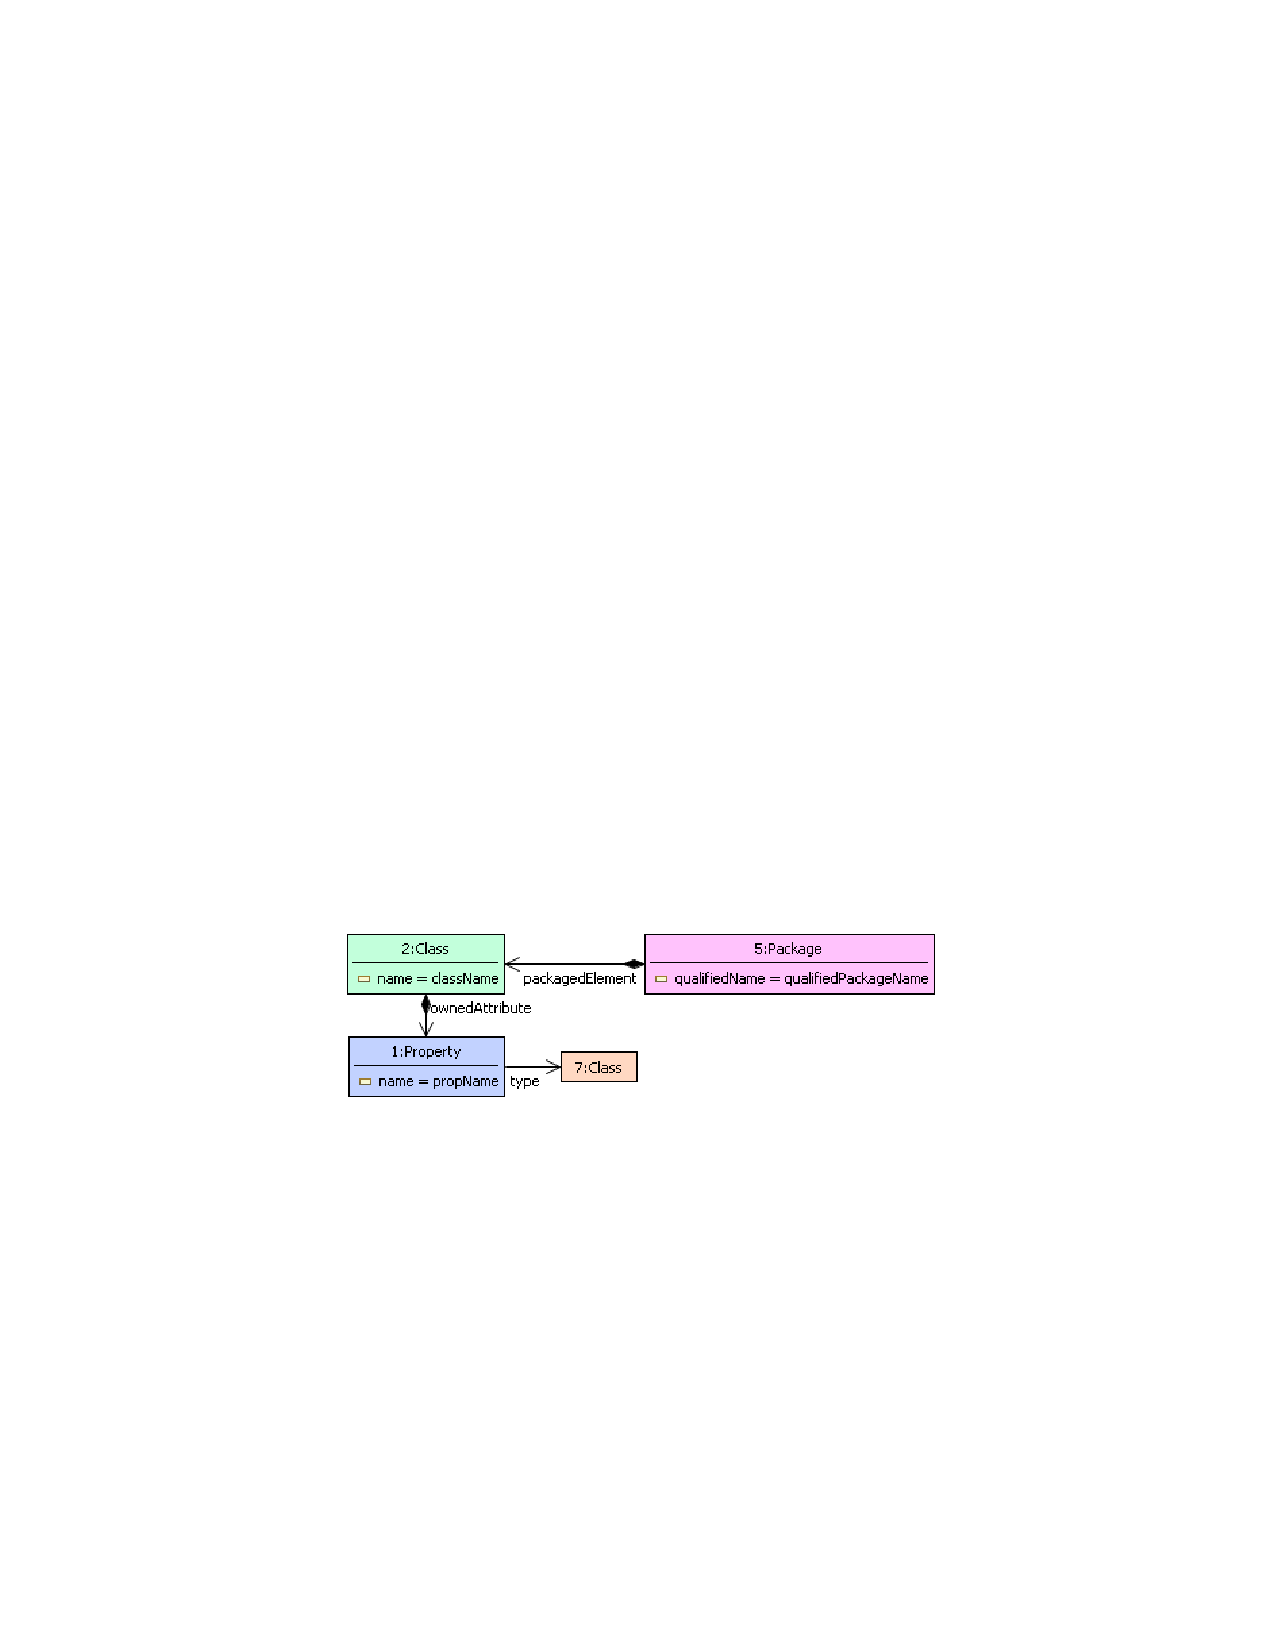
\includegraphics[width=11cm]{3.LiteratureReview/images/emf_refactor_lhs.pdf}
	}
	\subfigure[Right-hand side production rule.]
	{
	    \label{fig:emf_refactor_rhs}
	    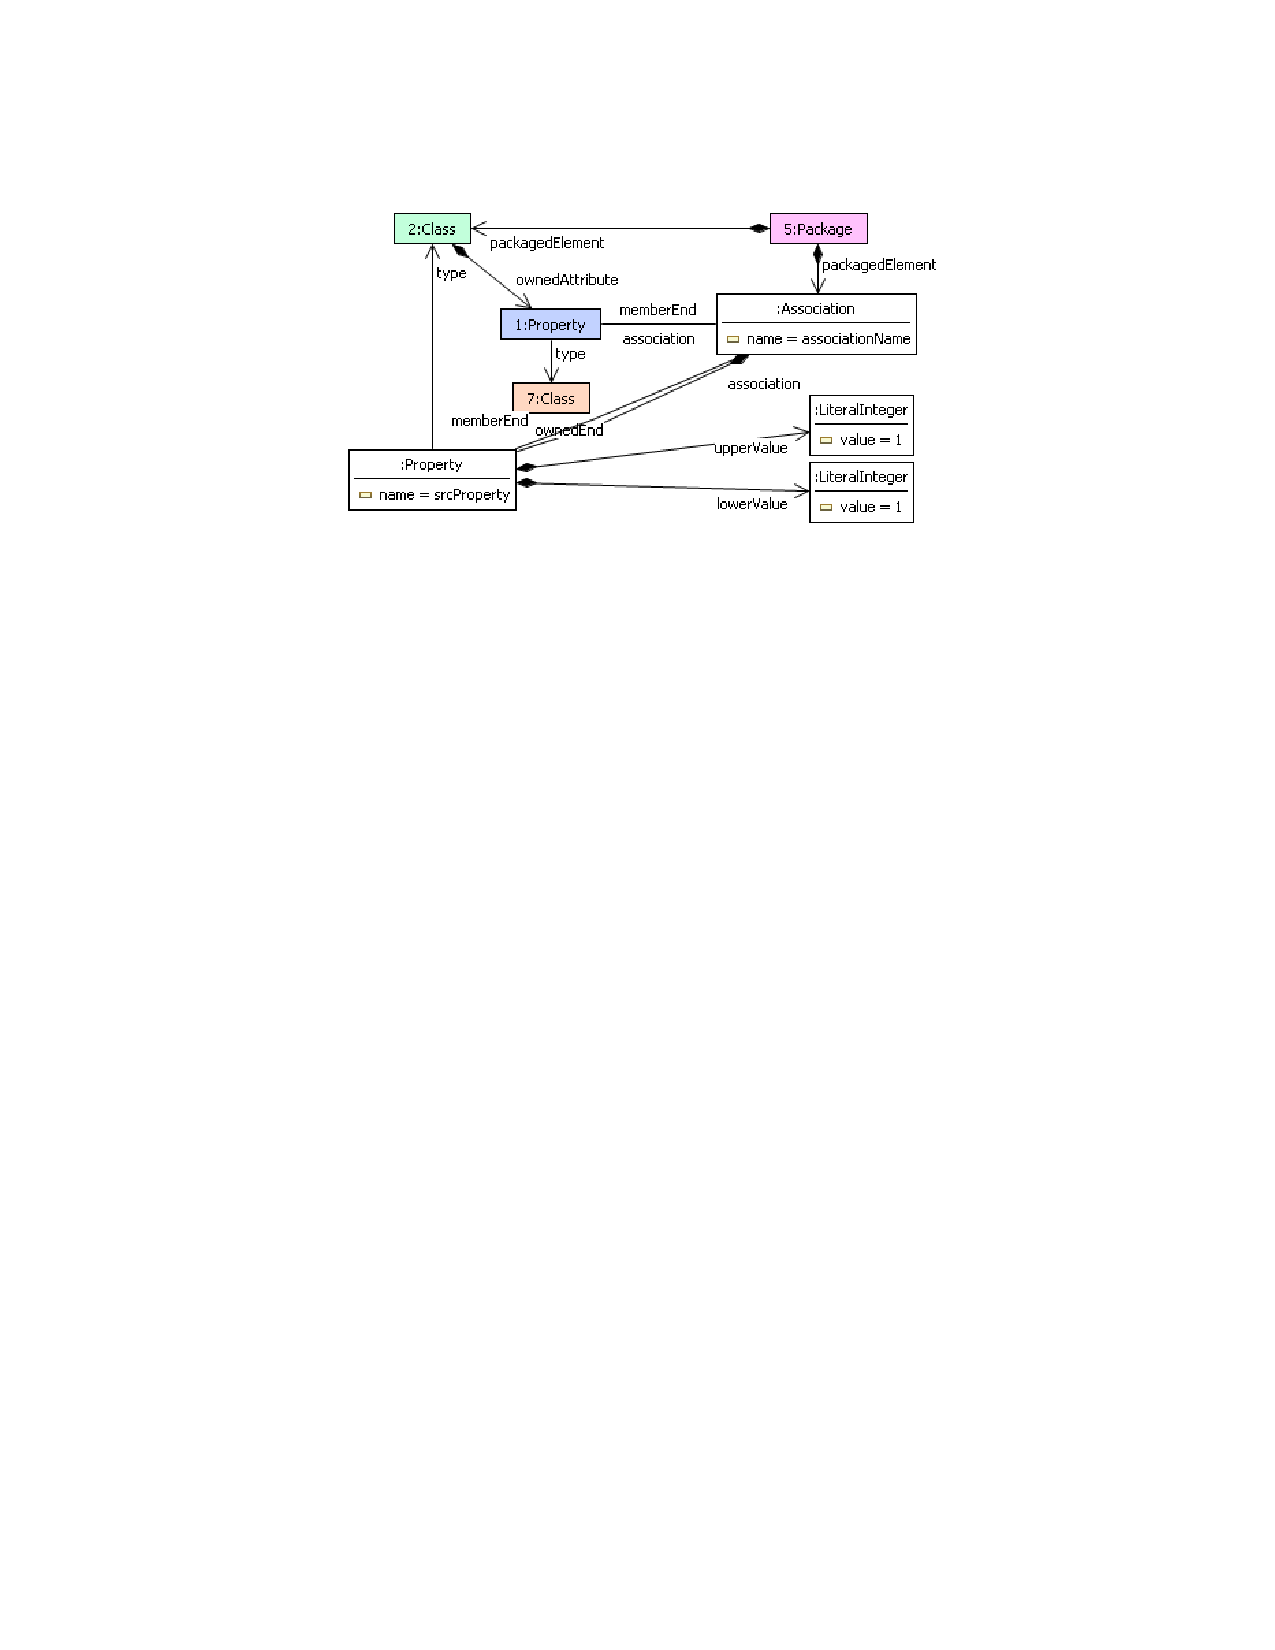
\includegraphics[width=12cm]{3.LiteratureReview/images/emf_refactor_rhs.pdf}
	}
	\caption[Attribute to association end refactoring in EMF Refactor]{Attribute to association end refactoring in EMF Refactor. Taken from \cite{arendt09refactoring}.}
\label{fig:emf_refactor}
\end{figure}

 
Existing model refactoring approaches focus on refactoring a model in isolation, rather than \emph{inter-model refactorings}, which affect more than one model at once. The Eclipse Java Development Tools support refactorings of Java code that update many source-code artefacts at once: for example, renaming a class in one source file updates references to that class in other source files. In \cc the context of MDE, support for inter-model refactoring would facilitate a greater degree of model modularisation and hence increase scalability, one of the key challenges for MDE \cite{kolovos08scalability}.

Model \cc refactoring research remains ``in its infancy'' \cite{mens07modelrefactoring}. Mens et al. identify formalisms for investigating the feasibility and scalability of model refactoring. In particular, Mens et al. suggest that meaning-preservation (an objective of refactoring, as discussed in Section \ref{subsec:refactoring}) can be checked by evaluating OCL constraints, behavioural models or downstream program code.


\subsubsection{Model Synchronisation}
\label{subsubsec:model_synch}
Changes made to development artefacts may require the \emph{synchronisation} of related artefacts (models, code, documentation). Traceability links (which capture the relationships of software artefacts) facilitate synchronisation. This section discusses the way in which change propagation is approached in the literature, which typically involves using an incremental style of transformation. Work that addresses more fundamental aspects of model synchronisation, such as capturing trace links and performing impact analysis are also discussed. Finally, synchronisation between models and text and between models and trace links is also considered.

\paragraph{Incremental transformation}
Many model synchronisation approaches extend or instrument existing model-to-model transformation languages. Declarative transformation languages are well-suited to the specification of bi-direct\-io\-nal transformations (which has been termed traceability-by-design \cite{fritzsche08tracing}) and \emph{incremental transformations}, a style of model transformation that facilitates incremental updates of the target model. In fact, much of the model synchronisation literature focuses on incremental transformation. 

Incremental transformation can be achieved in one of two ways. Because model-to-model transformation is used to generate one or more target models from one or more source models, when a source model changes, the model-to-model transformation can be invoked to completely re-generate the target models. This \cc activity has been termed \emph{re-transformation} and an alternative, \emph{live transformation}, in which the transformation context is persistent has been proposed \cite{hearnden06incremental}. Figure~\ref{fig:incremental_transformation_types} illustrates the differences between re-transformation and live transformation, showing the evolution of source and target models on the left-hand and right-hand sides, respectively, and the transformation context in the middle. Live transformation facilitates change propagation from the source to the target models without completely re-generating the target models and is therefore a more efficient approach when changes to the source models affect only part of the target models. Live \cc transformation appears to be a common way to achieve incremental transformation (e.g. \cite{rath08live,tratt08change}).

\begin{figure}[htbp]
	\centering
	\subfigure[Re-transformation.]
	{
	    \label{fig:re-transformation}
	    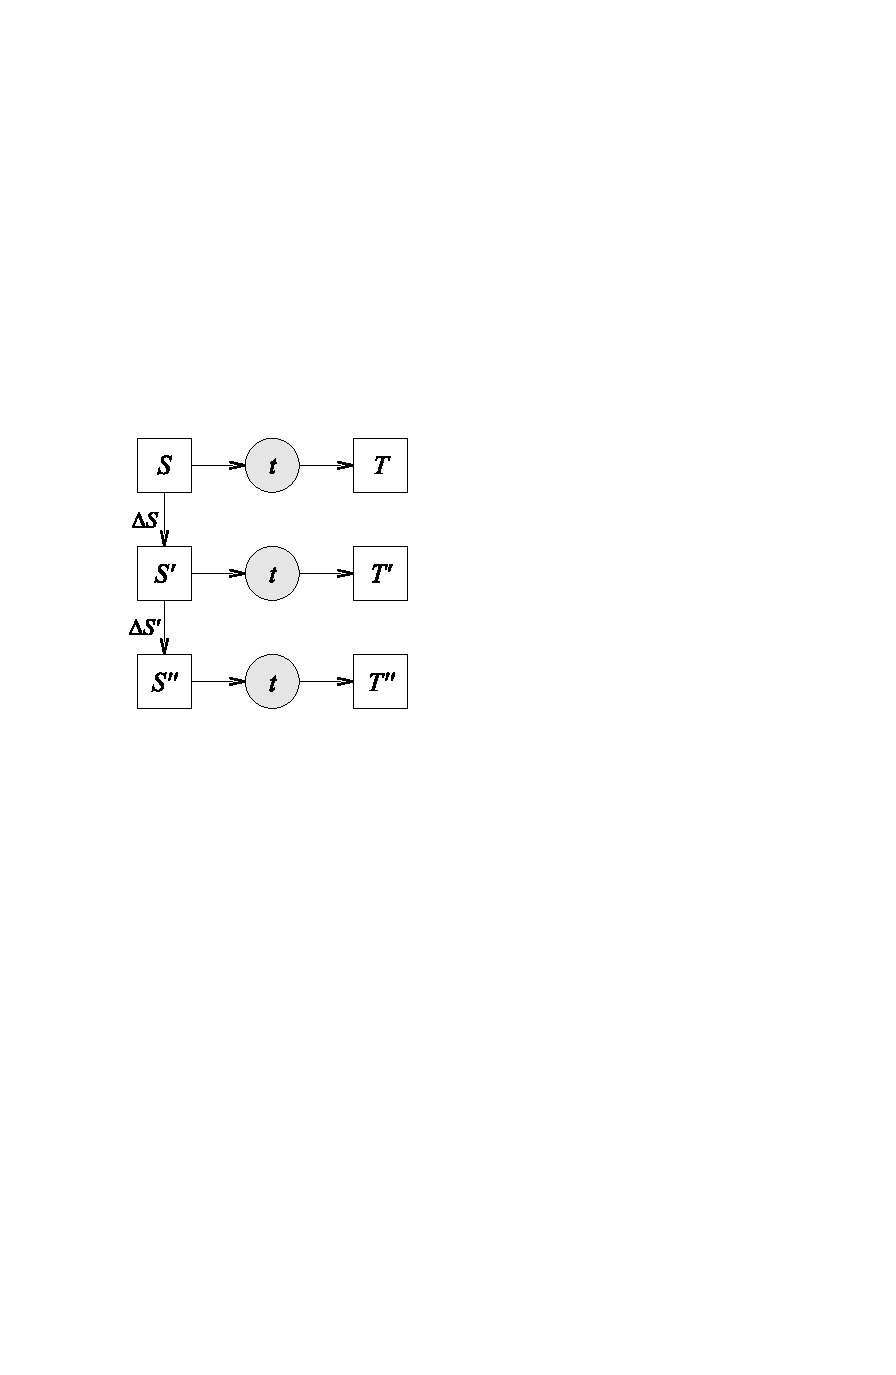
\includegraphics[width=5cm]{3.LiteratureReview/images/retransformation.pdf}
	}
	\subfigure[Live transformation.]
	{
	    \label{fig:live_transformation}
	    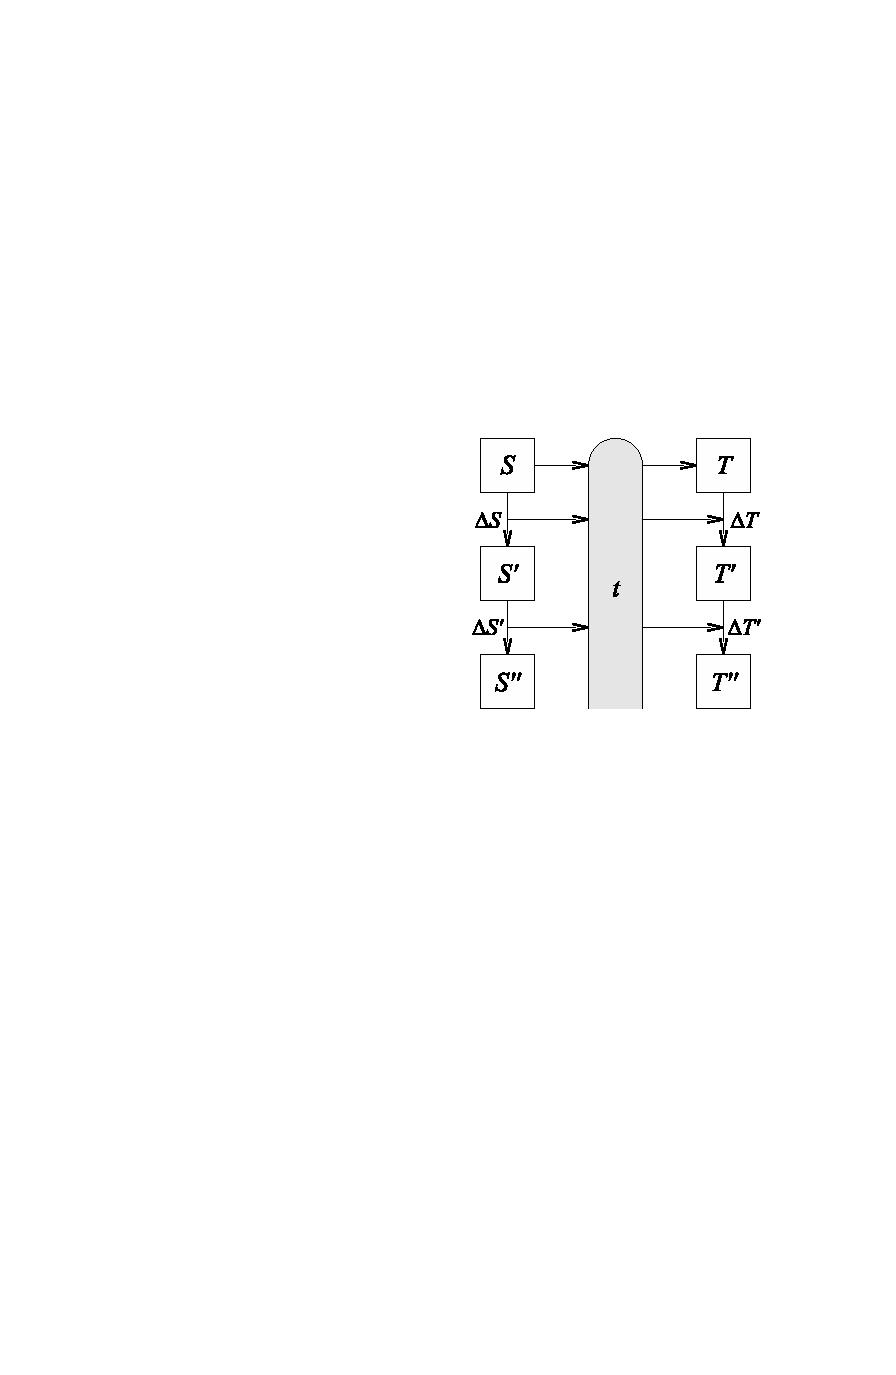
\includegraphics[width=5cm]{3.LiteratureReview/images/live_transformation.pdf}
	}
	\caption[Approaches to incremental transformation]{Approaches to incremental transformation. Taken from \cite{hearnden06incremental}.}
\label{fig:incremental_transformation_types}
\end{figure}

Primarily, incremental transformation has been used to address the scalability of model transformations. For large models, transformation execution time has been shown to be significantly reduced by using incremental transformation \cite{hearnden06incremental}. However, \cc it has been suggested that scalability should be addressed not only by attempting to develop techniques for increasing the speed of model transformation, but also by providing principles, practices and tools for building models that are less monolithic and more modular \cite{kolovos08scalability}. For this end, model synchronisation research should focus on maintainability as well as scalability.

Model \cc synchronisation and incremental transformation can be applied to decouple models and facilitate modularisation \cite{fritzsche08tracing}, although this is not commonly discussed in the literature. Fritzche et al. contribute a transformation that produces, from any UML model, a model for which performance characteristics can be readily analysed. The relationships between UML and performance model artefacts are recorded using traceability links. The results of the performance analysis are later fed back to the UML model using an incremental transformation made possible by the traceability links. Using this approach, performance engineers can focus primarily on the performance models, while other engineers are shielded from the low-level detail of the performance analysis. As such, Fritzsche et al. show that two different modelling concerns can be separated and decoupled, yet remain cohesive via the application of model synchronisation.

\paragraph{Towards automated model synchronisation}
Some existing work provides a foundation for automating model synchronisation activities. Theoretical aspects of the traceability literature were reviewed in Section~\ref{subsec:traceability}, and explored the automated activities that traceability facilitates, such as impact analysis and change propagation.  This section now analyses the traceability research in the context of MDE and focuses on the way in which traceability facilitates the automation of model synchronisation activities.

Aside from live transformation, other techniques for capturing trace links between models have been reported. To \cc this end, a model-to-model transformation has been enriched with traceability information using a generic higher-order transformation \cite{jouault05loosely}. Given a transformation, the generic higher-order transformation adds transformation rules that produce a traceability model. In \cc contrast to the genericity of the approach described by Jouault, Drivalos et al. propose domain-specific traceability metamodels for richer traceability link semantics \cite{drivalos08rigorously}. Further research is required to assess the requirements of automated model synchronisation tools and to select appropriate traceability approaches for their implementation.

Impact analysis is used to reason about the effects of a change to a development artefact. As well as facilitating change propagation, impact analysis can help to predict the cost and complexity of changes \cite{bohner02impactanalysis}. Impact analysis requires solutions to several sub-problems, which include change detection, analysis of the effects of a change, and effective display of the analysis.

Impact \cc analysis can be performed for UML models by comparing original and evolved versions of the same model to produce a report of evolved model elements that have been impacted by the changes to the original model elements \cite{briand03impactanalysis}. To facilitate the impact analysis, Briand \cc et al. identify change patterns that comprise, among other properties, a trigger (for change detection) and an impact rule (for marking model elements affected by this change). Figure~\ref{fig:impact_analysis_pattern} shows a sample impact analysis pattern for UML sequence diagrams, which is triggered when a message is added, and marks the sending class, the sending operation and the postcondition of the sending operation as impacted.

\begin{figure}[htbp]
  \begin{center}
    \leavevmode
    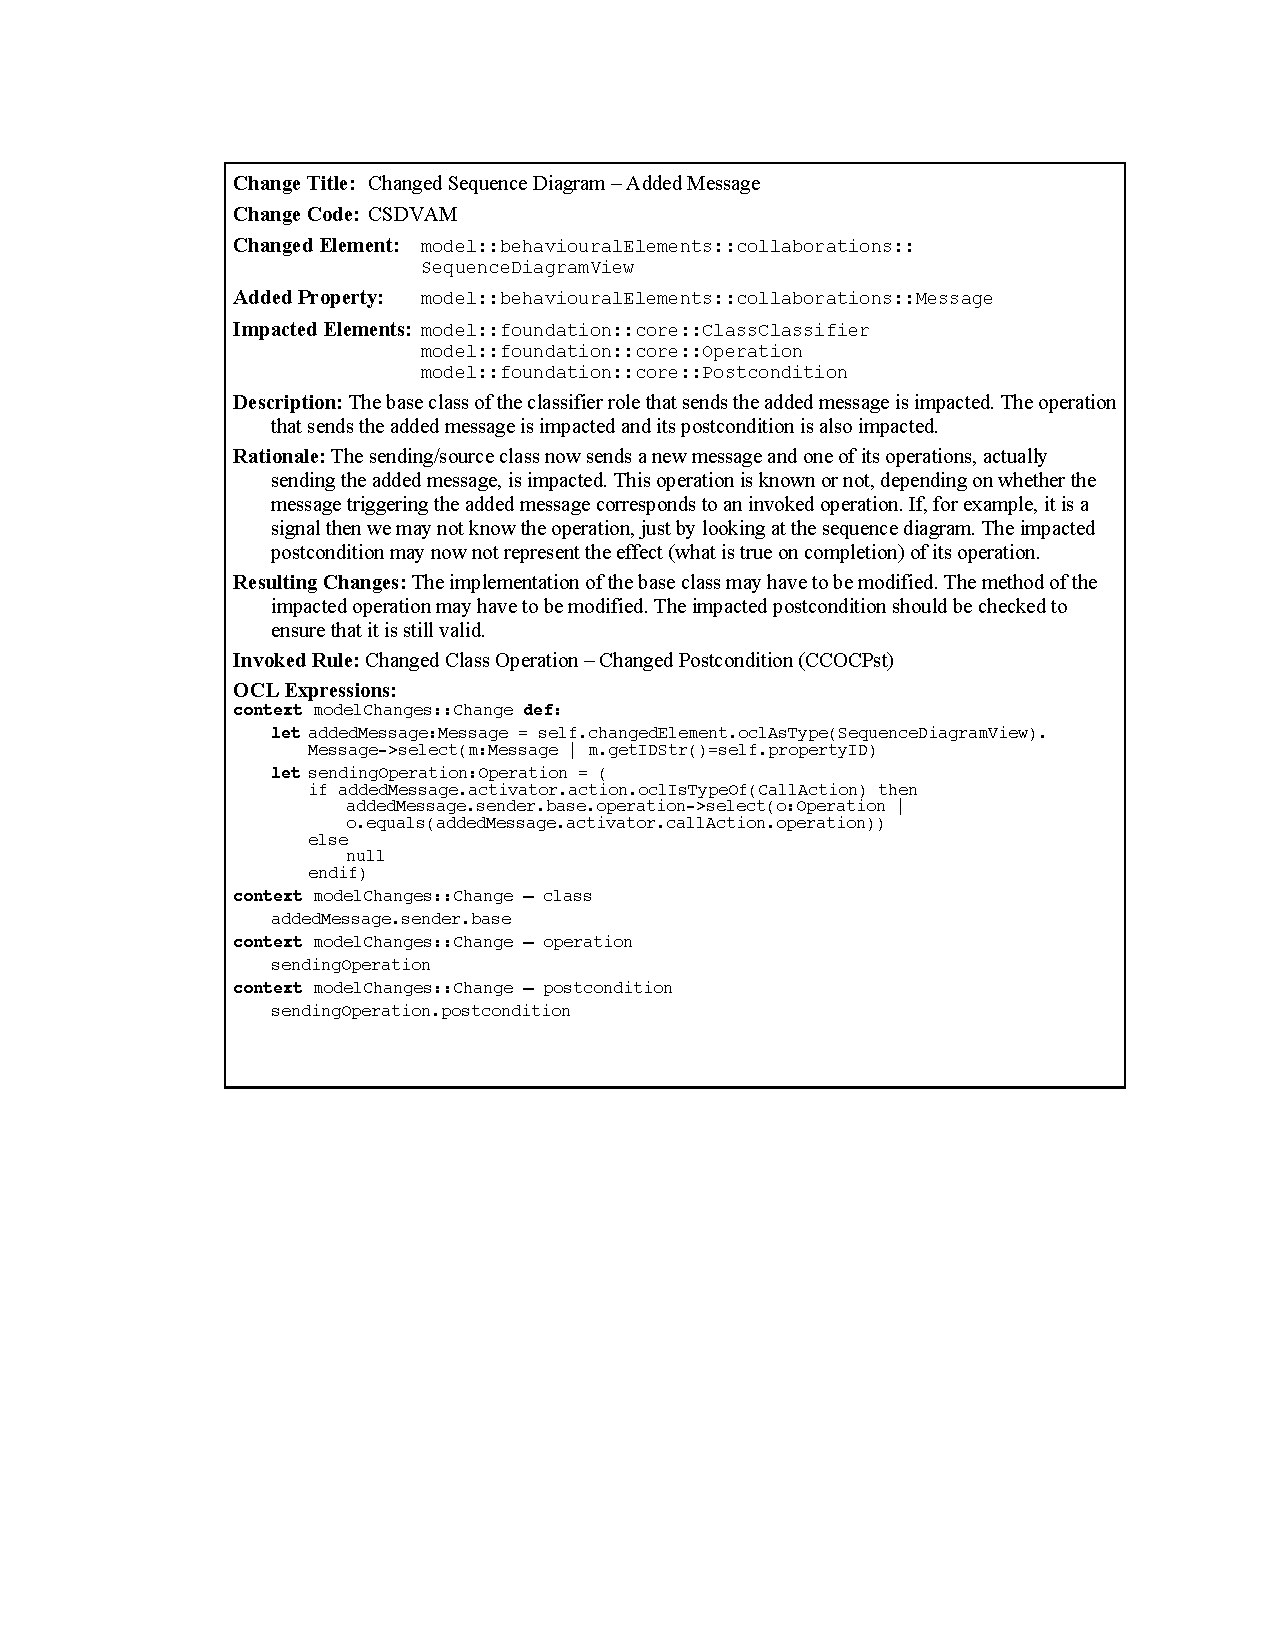
\includegraphics[width=12cm]{3.LiteratureReview/images/impact_analysis_pattern.pdf}
  \end{center}
  \caption[Example impact analysis pattern]{Example impact analysis pattern, taken from \cite{briand03impactanalysis}.}
  \label{fig:impact_analysis_pattern}
\end{figure}

Only \cc event-based approaches, such as the one described by Briand et al., have been proposed for automating impact analysis \cite{winkler09survey}. Because of the use of patterns for detecting changes and specifying resulting actions, event-based impact analysis is similar to differencing approaches for schema evolution (for example, \cite{lerner00model}, which was discussed in Section~\ref{subsec:schema_evolution}). When more than one trigger might apply, event-based impact analysis approaches must provide mechanisms for selecting between applicable patterns. The \cc selection policy used by Briand et al. is implicit (cannot be changed by the user) and does not provide a mechanism for selecting between applicable patterns.

Finally, model synchronisation tools might apply techniques used in automated synchronisation tools for traditional development environments. For example, the refactoring functionality of the Eclipse Java Development Tools \cite{fuhrer07refactoring} propagates changes between classes using a cache of the workspace to improve performance and scalability.


\paragraph{Synchronisation of models with text and trace links}
So far, this section has concentrated on model-to-model synchronisation, which is facilitated by traceability. Traceability is important for other software evolution activities in a model-driven development environment -- such as synchronisation between models and text and between models and trace links -- and these activities are now discussed.

While most of the model synchronisation literature focuses on synchronising models with other models, some papers consider synchronisation between models and other types of artefact. For synchronising changes in requirements documents with models, there is abundance of work in the field of requirements engineering, where the need for traceability was first reported. For synchronising models with generated text (during code generation, for example), the model-to-text language, Epsilon Generation Language (EGL) \cite{rose08egl}, produces traceability links between code generation templates and generated files. Sections of code can be marked protected, and are not overwritten by subsequent invocations of the code generation template. The MOFScript model-to-text language, like EGL, provides protected sections. Unlike EGL, MOFScript stores traceability links in a structured manner, facilitating impact analysis, model coverage (for highlighting which areas of the model contribute to the generated code) and orphan analysis (for detecting invalid traceability links) \cite{olsen07traceability}.

Trace links can be affected when development artefacts change. Synchronisation tools rely on accurate trace links and hence the maintenance of trace links is important. It \cc has been suggested that trace versioning should be used to address the challenges of trace link maintenance \cite{winkler09survey}, which include the accidental inclusion of unintended dependencies as well as the exclusion of necessary dependencies. Furthermore, \cc Winkler and von Pilgrim note that, although versioning traces has been explored in specialised areas (such as hypermedia \cite{nguyen05versioning}), there is no holistic approach for versioning traces.

\subsubsection{Model-metamodel Co-Evolution}
\label{LitReview:ModelCoEvo}
A metamodel describes the structures and rules for a family of models. When a model uses the structures and adheres to the rules defined by a metamodel, the model is said to \emph{conform} to the metamodel \cite{bezivin05unification}. A change to a metamodel might require changes to models to ensure the preservation of conformance. The process of evolving a metamodel and its models together to preserve conformance is termed \emph{model-metamodel co-evolution} and is subsequently referred to as \emph{co-evolution}. This section explores existing approaches to co-evolution, comparing them with work from the closely related areas of schema and grammar evolution approaches (Sections~\ref{subsec:schema_evolution} and \ref{subsec:grammar_evolution}). A more thorough analysis of co-evolution approaches is conducted in Chapter~\ref{Analysis}.

\paragraph{Co-evolution theory}
A co-evolution process involves changing a metamodel and updating instance models to preserve conformance. Often, the two activities are considered separately, and the latter is termed \emph{migration}. In this thesis, the term \emph{migration strategy} is used to mean an algorithm that specifies migration. Sprinkle \cc and Karsai were the first to identify the need for approaches that consider the specific requirements of co-evolution \cite{sprinkle04domain}. In particular, Sprinkle and Karsai describe migration as distinct from -- and as having unique challenges compared to -- the more general activity of model-to-model transformation. The \cc phrase ``evolution, not revolution'' has been used to highlight and emphasise that, during co-evolution, the difference between source and target metamodels is often small \cite{sprinkle03thesis}.

Understanding the situations in which co-evolution must be managed is important for formulating appropriate requirements for co-evolution tools. Migration \cc is sometimes made unnecessary by evolving a metamodel such that the conformance of models is not affected (for example, making only additive changes) \cite{herrmannsdoerfer09cope}. Co-evolution \cc can be carried out by more than one person, and in some cases metamodel developers and model users might not communicate \cite{cicchetti08automating}. Notwithstanding these observations, the co-evolution literature rarely reports on the ways in which co-evolution is managed in practice. 

\paragraph{Co-evolution patterns}
Much of the co-evolution literature suggests that the way in which migration is performed should vary depending on the type of metamodel changes made \cite{gruschko07towards,herrmannsdoerfer09cope,cicchetti08automating,garces09managing}. In particular, the co-evolution literature identifies two important classifications of metamodel changes that affect the way in which migration is performed. Depending \cc on the type of metamodel change, migration might be unnecessary (\emph{non-breaking} change), can be automated (\emph{breaking and resolvable} change) and can be automated only when ambiguity is resolved by a developer (\emph{breaking and non-resolvable} change) \cite{gruschko07towards}. Metamodel \cc changes can also be regarded as either \emph{metamodel-independent} (observed in the evolution of more than one metamodel) or \emph{metamodel-specific} (observed in the evolution of only one metamodel) \cite{herrmannsdoerfer08automatability}.

Further research is needed to identify categories of metamodel changes, because many automated co-evolution approaches are underpinned by the categorisations. It \cc has been suggested that a large proportion of metamodel changes re-occur \cite{herrmannsdoerfer08automatability}, but the study in which this claim was made considers only two metamodels, both taken from the same organisation. Assessing the extent to which changes re-occur across a larger and broader range of metamodels is an open research challenge to which this thesis contributes, particularly in Chapter~\ref{Analysis}.

\paragraph{Co-evolution approaches}
Several approaches for managing co-evolution have been proposed, most of which are based on one of the two classifications of metamodel changes described above.

Re-use \cc of migration knowledge is a primary concern in the work of Herrmannsd\"{o}rfer, which is premised on an observation that a large proportion of metamodel changes re-occurred during the development of two metamodels \cite{herrmannsdoerfer08automatability}. COPE \cc \cite{herrmannsdoerfer09cope} is a co-evolution tool that provides a library of co-evolutionary operators. Operators are applied to evolve a metamodel and have pre-defined migration semantics. The application of each operator is recorded, and used to generate an executable migration strategy. Due to its use of re-usable operators, COPE shares characteristics with operator-based approaches for schema and grammar evolution (Sections~\ref{subsec:schema_evolution} and \ref{subsec:grammar_evolution}). Consequently, the limitations of operator-based schema evolution approaches \cite{lerner00model} apply to COPE. Balancing expressiveness and understandability is a key challenge for operator-based approaches because the former implies a large number of operators while the latter a small number of operators.

Gruschko et al. suggest inferring co-evolution strategies, based on either a difference model of two versions of the evolving metamodel (direct comparison) or on a list of changes recorded during the evolution of a metamodel (indirect comparison) \cite{gruschko07towards}. To this end, Gruschko et al contribute the co-evolution process shown in Figure \ref{fig:coevoprocess}. 

\begin{figure}[htbp]
  \begin{center}
    \leavevmode
    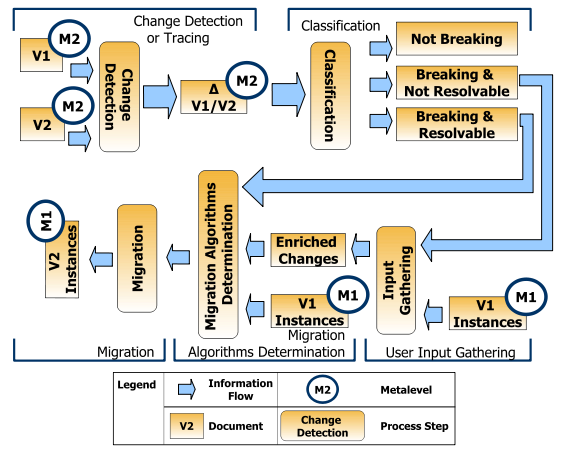
\includegraphics[scale=0.6]{3.LiteratureReview/images/CoEvoProcess.png}
  \end{center}
  \caption[An exemplar co-evolution process]{The co-evolution process described in \cite{gruschko07towards}.}
  \label{fig:coevoprocess}
\end{figure}

Two \cc inference approaches inspired by the work of Gruschko et al. are now described. Both approaches use a co-evolution process similar to the one shown in Figure \ref{fig:coevoprocess}, and use higher-order model transformation\footnote{A model-to-model transformation that consumes or produces a model-to-model transformation is \emph{higher-order}.} for determining the migration strategy (the penultimate phase in Figure~\ref{fig:coevoprocess}). Cicchetti \cc et al. contribute a metamodel for describing the similarities and differences between two versions of a metamodel, enabling a model-driven approach to generating model migration strategies \cite{cicchetti08automating}. Garc\'{e}s \cc et al. provide a similar metamodel, but use a metamodel matching process that can be customised by the user, who specifies matching heuristics to form a matching strategy \cite{garces09managing}. Otherwise, the co-evolution approaches described by Cicchetti et al. and Garc\'{e}s et al. are fully automatic and cannot be guided by the user. Clearly \cc then, accuracy is important for approaches that compare two metamodel versions, but Cicchetti et al. and Garc\'{e}s et al. do not explore the extent to which the proposed approaches can be applied.

Some co-evolution approaches predate the classifications of metamodel changes described above. For instance, a \cc preliminary catalogue of metamodel changes was the first to employ higher-order transformation for specifying model migration \cite{wachsmuth07metamodel}. However, Wachsmuth \cc considers a small number of metamodel changes occurring in isolation and, as such, it is not clear whether the approach can be used in the general case. Sprinkle \cc proposes a visual transformation language for specifying model migration based on graph transformation theory \cite{sprinkle03thesis}, which is less expressive than imperative or hybrid transformation languages (as discussed in Section~\ref{subsubsec:model_transformation}).

\subsubsection{Visualisation}
To better understand the effects of evolution on development artefacts, visualising different versions of each artefact may be beneficial. Existing research for comparing text can be enhanced to perform semantic-differencing of models with a textual concrete syntax. For models with a visual concrete syntax, another approach is required. 

To \cc visualise the way in which model elements are transformed by transformation chains (the sequential composition of model-to-model transformations), a three-dimensional editor has been implemented \cite{pilgrim08constructing}. Figure \ref{fig:transformation-chains} depicts a sample transformation chain visualisation. Each plane represents a model. The links between each plane illustrates the effects of a model-to-model transformation. The visualisation style used in the three-dimensional editor could be used to facilitate exploration of artefact evolution.


\begin{figure}[htbp]
  \begin{center}
    \leavevmode
    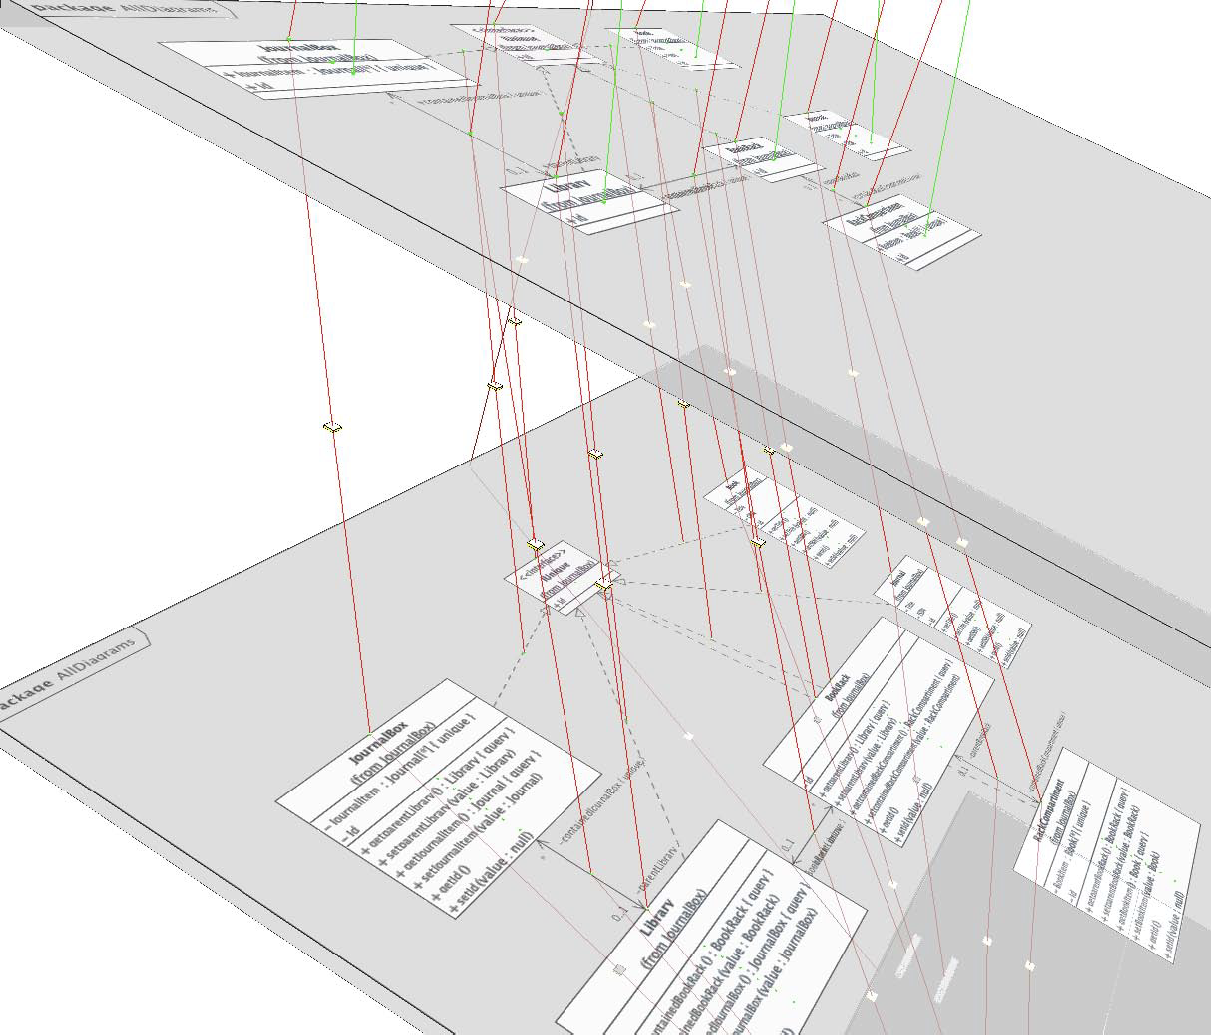
\includegraphics[scale=0.25]{3.LiteratureReview/images/transformation-chain.png}
  \end{center}
  \caption[Visualising a transformation chain]{Visualising a transformation chain. Taken from \cite{pilgrim08constructing}.}
  \label{fig:transformation-chains}
\end{figure}

\paragraph{Summary}
Fully automated migration is still an open research challenge. Co-evolution approaches are in their infancy, and key problems need to be addressed. For \cc example, matching schemas (metamodels) can yield more than one feasible set of migration strategies \cite{lerner00model}. To this end, matching \cc heuristics, which guide the inference of the model migration strategy -- but might affect the predictability of the co-evolution process -- have been proposed \cite{garces09managing}. 

Another open research challenge is in identifying an appropriate notation for describing migration. Existing \cc tools use higher-order transformations \cite{wachsmuth07metamodel,cicchetti08automating} or general-purpose programming languages \cite{herrmannsdoerfer09cope}. Migration is a specialisation of model-to-model transformation \cite{sprinkle04domain}, and therefore languages other than model-to-model transformation languages might be more suitable for describing migration.

Until co-evolution tools reach maturity, improving MDE modelling frameworks to better support co-evolution is necessary. For example, EMF (Section~\ref{subsec:emf}) cannot load models that no longer conform to their metamodel and, hence non-conformant models cannot be loaded in model editors, and cannot be used with model management operations.

This section has surveyed the existing work on identifying and managing software evolution in the context of MDE. In particular, several types of evolutionary change to modelling artefacts have been identified. Chapter~\ref{Analysis} provides a more detailed and critical analysis of the work described in this section. In particular, Section~\ref{sec:analysing_existing_techniques} compares different approaches to managing co-evolution using an example from an MDE project.

\section[Challenges to Managing Software Evolution in MDE][Challenges to Managing Evolution in MDE]{Challenges to Managing Software Evolution in MDE}
From the review presented above, several research challenges for managing software evolution in the context of MDE are synthesised. The challenges summarised in this section were considered as possible research directions for the thesis research.

\paragraph{Model refactoring challenges} The model refactoring literature proposes tools and techniques for improving the quality of existing models without affecting their functional behaviour. In traditional development environments, inter-artefact refactoring (in which changes span more than one development artefact) is often automated, but none of the model refactoring papers discussed in this chapter consider inter-model refactoring. In general, the refactoring literature covers several concerns, such as identification, validation and assessment (Section~\ref{subsec:refactoring}), but the model refactoring literature considers only the specification and application of refactoring. To better understand the costs and benefits of model refactoring, further model refactoring research must also explore the identification, validation and assessment of model refactorings.

\paragraph{Model synchronisation challenges} Improved \cc scalability is the primary motivation of most model synchronisation research, although it has been suggested that model synchronisation can be used to improve the maintainability of a system via modularisation \cite{fritzsche08tracing}. Consequently, further research should explore the extent to which model synchronisation can be used to manage evolution. For impact analysis between models, only event-based approaches have been reported; other approaches -- used successfully to manage evolution in other fields (such as relational databases and grammarware) -- have not been applied to models \cite{winkler09survey}. Few papers consider synchronisation with other artefacts and maintaining trace links and there is potential for further research in these areas.

\paragraph{Model-metamodel co-evolution challenges} To better understand model-metamodel co-evolution, further studies of the ways in which metamodels change are required. The \cc existing empirical study of industrial metamodels \cite{herrmannsdoerfer08automatability} focuses only on two metamodels produced in the same organisation. Challenges for co-evolution reported in other fields have not been addressed by the model-metamodel co-evolution literature. For \cc example, comparing two versions of a changed artefact (such as metamodel) can suggest more than one feasible migration strategy \cite{lerner00model}. Approaches to co-evolution that do not consider the way in which a metamodel has changed, such as \cite{cicchetti08automating,garces09managing}, must address this challenge. A range of notations are used for model migration, including model-to-model transformation languages and general-purpose programming languages, which is a challenge for the comparison of co-evolution tools. Finally, contemporary MDE modelling frameworks do not facilitate MDE for non-conformant models, which is problematic at least until co-evolution tools reach maturity.  

\paragraph{General challenges for evolution in MDE} From the analysis in this chapter, several research challenges for software evolution in the context of MDE are apparent. Greater understanding of the situations in which evolution occurs informs the identification and management of evolution, yet few papers study evolution in real-world MDE projects. Analysis of existing projects can yield patterns of evolution, providing a common vocabulary for thinking and communicating about evolution. These patterns are used as a foundation \changed{``built atop'' changed to ``used as a foundation'' by rephrasing sentence} for notations and tools used to automate some evolution activities. In addition, recording, analysing and visualising changes made over the long term to MDE development artefacts and to MDE projects is an area that is not considered in the literature.

\section{Chapter Summary}
\label{sec:literature_review_summary}
This chapter has reviewed and analysed software evolution literature. Two evolution activities explored in the remainder of this thesis, \emph{impact analysis} and \emph{change propagation}, were introduced. Principles and practices of software evolution (from the fields of programming languages, relational database systems and grammarware) were compared and analysed. In particular, software evolution literature from the MDE community was reviewed and analysed to allow the synthesis of research challenges and potential directions for the thesis research.

As well as directing the thesis research, the literature review influenced the choice of research method. Most of the software evolution research discussed in this chapter (such as \cite{guerrini05impact,kramer01xem,su01xem} for XML schema evolution and \cite{banerjee87semantics,edelweiss05temporal} for relational database schema evolution) uses a similar method: first, identify and categorise evolutionary changes by considering all of the ways in which artefacts can change. Next, design a taxonomy of operators that capture these changes or a matching algorithm that detects the application of the changes. Then, implement a tool for applying operators, invoking a matching algorithm, or trigger change events. Finally, evaluate the tool on existing projects containing examples of evolution. This method assumes that most (if not all) evolutionary changes can be identified and captured from existing examples of evolution, and does not consider the ways in which evolution is already managed in existing projects. An alternative method was used to conduct the thesis research, which was discussed in Section~\ref{sec:research_method} and based on the method used by Dig in his work on program refactoring (\cite{dig07thesis}). First, existing projects were analysed to better understand the situations in which evolution occurs. From this analysis, research requirements were derived, and structures and processes for managing evolution were implemented. The structures and processes were evaluated by comparison with related structures and processes, and by application to real-world MDE projects in which evolution had occurred. This method was preferred as existing work on evolution in MDE (Section~\ref{subsec:mde_evo}) does not consider the way in which evolution is managed in existing MDE projects, and, with the exception of COPE \cite{herrmannsdoerfer09cope}, can only be used to manage a fixed set of evolutionary changes.

The review and the research challenges presented in this chapter led to a critical analysis of techniques for identifying and managing evolution in the context of software evolution. Chapter~\ref{Analysis} presents the critical analysis, which was conducted using examples from real-world MDE projects.